\subsection{亏格二}%
\label{sub:Genus two}

这里讨论的亏格二镜像公式出自 Guo--Janda--Ruan~\cite{GJRgenus2}。

现在我们在亏格二中同时执行两条路线。几何路线使用 \(t\)-扭曲稳定商理论，先用虚拟局部化得到五项贡献，再用稳定商越墙（wall-crossing）过渡到五次格罗莫夫–威滕理论。形式路线则使用半单的 \(\lambda\)-扭曲理论和 \(R\)-矩阵来计算稳定图和。这只给出形式主部，之后还必须补上有效与亚纯的其余图（rest graphs）。

\begin{notn}
    记
    \[ \ab<\alpha_1, \ldots, \alpha_n>^{t,\mr{SQ}}_{g,n} \coloneqq \sum_{d\geq0}q^d \int_{[\Mbar_{g,n}(\P^4,d)]^{\vir}}e(R\pi_*\mc{L}^{\otimes 5}\otimes[-1])\prod_i \ev_i^*(\alpha_i), \]
    其中 \(\mc{L}\) 是泛稳定商线丛，且 \(c_1^{\C^{\times}}([-1]) = -t\)（这一符号约定下文还会再提到）。这是稳定商的符号约定，与上文稳定映射圈中出现的 \([1]\) 并不相同。
\end{notn}

\begin{figure}[htpb]
    \centering
    \begin{tikzpicture}[scale=0.95,transform shape]
        \draw[gray] (-0.9,0) -- (11.2,0);
        \draw[gray] (-0.9,2.2) -- (11.2,2.2);
        \node[anchor=east,gray] at (-0.9,0) {$0$};
        \node[anchor=east,gray] at (-0.9,2.2) {$\infty$};
        \node[ellipse,draw,thick,minimum width=1.5cm,minimum height=0.75cm] (a) at (0,0) {$\Sigma_2(d)$};
        \node at (0,-1) {$\Gamma^2$};
        \node[ellipse,draw,thick,minimum width=1.5cm,minimum height=0.75cm] (b0) at (2.7,0) {$\Sigma_1(d)$};
        \node[ellipse,draw,thick,minimum width=1.5cm,minimum height=0.75cm] (b1) at (2.7,2.2) {$\Sigma_1(0)$};
        \draw[thick] (b0) -- (b1);
        \node at (2.7,-1) {$\Gamma^1$};
        \node[ellipse,draw,thick,minimum width=1.5cm,minimum height=0.75cm] (c0) at (5.6,0) {$\Sigma_0(d)$};
        \node[ellipse,draw,thick,minimum width=1.5cm,minimum height=0.75cm] (c1) at (4.9,2.2) {$\Sigma_1(0)$};
        \node[ellipse,draw,thick,minimum width=1.5cm,minimum height=0.75cm] (c2) at (6.6,2.2) {$\Sigma_1(0)$};
        \draw[thick] (c0) -- (c1);
        \draw[thick] (c0) -- (c2);
        \node at (5.6,-1) {$\Gamma_b^0$};
        \node[ellipse,draw,thick,minimum width=1.5cm,minimum height=0.75cm] (d0) at (9.6,0) {$\Sigma_0(d)$};
        \node[ellipse,draw,thick,minimum width=1.5cm,minimum height=0.75cm] (d1) at (9.6,2.2) {$\Sigma_1(0)$};
        \draw[thick] (d0) to[bend left=25] (d1);
        \draw[thick] (d0) to[bend right=25] (d1);
        \node at (9.6,-1) {$\Gamma_a^0$};
    \end{tikzpicture}
    \caption{亏格二中四个非常值的局部化图，每个顶点画成其对应的黎曼面分支。}%
    \label{fig:g2loc}
\end{figure}

四个非常值图见~\Cref{fig:g2loc}，其贡献为
\begin{align*}
    \Cont_{\Gamma^2} &= \ab<>^{t,\mr{SQ}}_{2,0}, \\
    \Cont_{\Gamma^1} &= -\ab< \frac{-\frac{5}{2}H^3 + \frac{5}{24}H^4t^{-1}}{(t-5H)(t-5H-\psi)}>^{t,\mr{SQ}}_{1,1}, \\
    \Cont_{\Gamma_b^0} &= \ab< \frac{-\frac{5}{2}H^3+\frac{5}{24}H^4t^{-1}}{(t-5H)(t-5H-\psi_1)}, \frac{-\frac{5}{2}H^3+\frac{5}{24}H^4t^{-1}}{(t-5H)(t-5H-\psi_2)}>^{t,\mr{SQ}}_{0,2},
\end{align*}
对双边图记 \(H_1 = H \otimes 1\)、\(H_2 = 1 \otimes H\)，则
\[ \Cont_{\Gamma_a^0} = \ab< \frac{\frac{5}{3}(H^3\otimes H^4 + H^4 \otimes H^3)t^{-1} + \frac{65}{24}H^4 \otimes H^4 t^{-2}}{(t-5H_1)(t-5H_1-\psi_1)(t-5H_2)(t-5H_2-\psi_2)}>^{t,\mr{SQ}}_{0,2}. \]
注意到这些关联子是在 \(\P^4\) 上取的，故其中 \(H^4\) 出现且非零。

第五项贡献来自零次图，即常数
\[ -2c_{2,0} = -\frac{5}{144}, \qquad c_{2,0} = -\frac{1}{2}N_{2,0} = \frac{5}{288}, \]
把这五项贡献相加，我们得到局部化恒等式
\[ F_2^{\mr{SQ}}(q) = \Cont_{\Gamma^2} + \Cont_{\Gamma^1} + \frac{1}{2}\Cont_{\Gamma_a^0} + \frac{1}{2}\Cont_{\Gamma_b^0} - 2c_{2,0}, \]
其中两个 \(\frac{1}{2}\) 因子来自 \(\Gamma_a^0\) 与 \(\Gamma_b^0\) 的自同构。

设 \(Q = qe^{\tau(q)}\)、\(L = (1-5^5q)^{-1/5}\)，其中 \(\tau(q) = I_1(q)/I_0(q) - \log q\) 是通常的镜像平移。现在应用稳定商越墙，得到精确恒等式
\[ F_2^{\mr{GW}}(Q) = I_0(q)^2 F_2^{\mr{SQ}}(q). \]
引入 \(D_u = L^{-1}q\odv{}{q}\) 以及生成元
\[ \mc{X}_k = D_u^k \log \frac{I_0}{L}, \qquad \mc{Y}_k = D_u^k \log \frac{I_0I_{1,1}}{L^2}, \qquad I_{1,1} = 1 + q \odv{\tau}{q}, \quad D_u L = \frac{1}{5}(L^5-1), \]
各个扭曲图的贡献还涉及额外的生成元。对我们来说关键的一点是：这些生成元在上述线性组合中相互抵消，恰好留下有限生成变量。记 \(X = \mc{X}_1\)、\(Y_1 = \mc{Y}_1\)，我们得到
\begin{align*}
    F^{\mr{GW}}_2(Q) = \frac{I_0^2}{L^2}\Big(&\frac{70}{9}\mc{X}_3 + \frac{575}{18}X\mc{X}_2 + \frac{557}{72}X^3 + \frac{5}{6}Y_1\mc{X}_2 \\
    &- \frac{629}{72}Y_1X^2 - \frac{23}{24}Y_1^2 X - \frac{1}{24}Y_1^3 \\
    &+ \frac{125}{36}\mc{X}_2 L^4 - \frac{5}{24}X^2L^4 - \frac{35}{9}Y_1XL^4 - \frac{5}{24}Y_1^2L^4 \\
    &- \frac{1441}{300}XL^3 - \frac{41}{300}Y_1L^3 + \frac{31459}{7200}XL^8 + \frac{2141}{7200}Y_1L^8 \\
    &+ \frac{29621}{12000}L^{12} - \frac{116369}{36000}L^7 + \frac{547}{750}L^2\Big).
\end{align*}
在大半径处展开，我们得到
\[ F_2^{\mr{GW}}(Q) = -\frac{5}{144} + \frac{575}{48}Q + \frac{5125}{2}Q^2 + \frac{7930375}{6}Q^3 + O(Q^4), \]
这些系数是格罗莫夫–威滕不变量 \(N_{2,d}\)，而非~\Cref{tab:quinticbps} 中的 BPS 整数。

现在转向形式路线。\(\Omega^{\lambda}_{2,0}\) 的 Givental-Teleman 公式是对无腿的七个亏格二稳定图求和，这些图见~\Cref{fig:g2stable}。只需用到 \(R^{-1}(z)\) 直到 \(z^3\) 的部分，而平移把这七种拓扑展开成 \(17\) 个带装饰的层（strata）。

\begin{figure}[htpb]
    \centering
    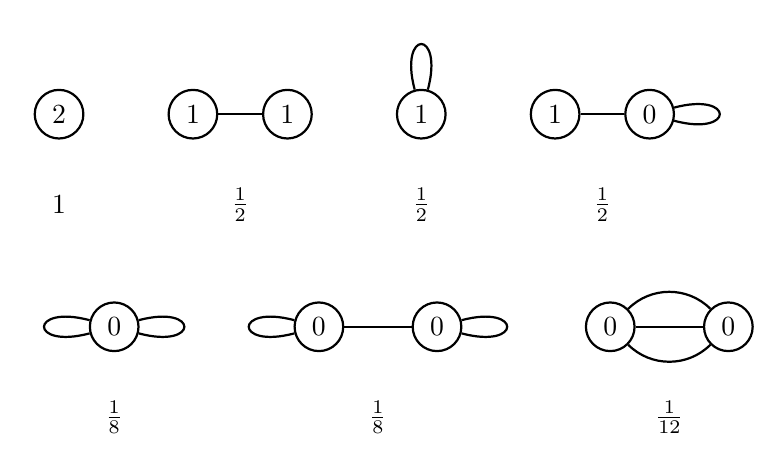
\begin{tikzpicture}[scale=1,transform shape,every loop/.style={min distance=8mm,looseness=10}]
        \node[circle,draw=black,thick] (a) at (0,0) {$2$};
        \node at (0,-1.15) {$1$};

        \node[circle,draw=black,thick] (b1) at (1.7,0) {$1$};
        \node[circle,draw=black,thick] (b2) at (2.9,0) {$1$};
        \draw[thick] (b1) -- (b2);
        \node at (2.3,-1.15) {$\frac{1}{2}$};

        \node[circle,draw=black,thick] (c) at (4.6,0) {$1$};
        \draw[thick] (c) edge[loop above] (c);
        \node at (4.6,-1.15) {$\frac{1}{2}$};

        \node[circle,draw=black,thick] (d1) at (6.3,0) {$1$};
        \node[circle,draw=black,thick] (d2) at (7.5,0) {$0$};
        \draw[thick] (d1) -- (d2);
        \draw[thick] (d2) edge[loop right] (d2);
        \node at (6.9,-1.15) {$\frac{1}{2}$};

        \node[circle,draw=black,thick] (e) at (0.7,-2.7) {$0$};
        \draw[thick] (e) edge[loop left] (e);
        \draw[thick] (e) edge[loop right] (e);
        \node at (0.7,-3.85) {$\frac{1}{8}$};

        \node[circle,draw=black,thick] (f1) at (3.3,-2.7) {$0$};
        \node[circle,draw=black,thick] (f2) at (4.8,-2.7) {$0$};
        \draw[thick] (f1) -- (f2);
        \draw[thick] (f1) edge[loop left] (f1);
        \draw[thick] (f2) edge[loop right] (f2);
        \node at (4.05,-3.85) {$\frac{1}{8}$};

        \node[circle,draw=black,thick] (g1) at (7.0,-2.7) {$0$};
        \node[circle,draw=black,thick] (g2) at (8.5,-2.7) {$0$};
        \draw[thick] (g1) -- (g2);
        \draw[thick] (g1) to[bend left=45] (g2);
        \draw[thick] (g1) to[bend right=45] (g2);
        \node at (7.75,-3.85) {$\frac{1}{12}$};
    \end{tikzpicture}
    \caption{无腿的七个亏格二稳定图，顶点处标以其亏格，并赋以权 \(\frac{1}{\ab|\Aut\Gamma|}\)。在幻灯片中每个顶点都画成其对应的黎曼面分支。}%
    \label{fig:g2stable}
\end{figure}

\begin{rmk}
    这些是稳定曲线的对偶图，并非~\Cref{fig:tropgraphs} 中的图；后者是把热带分解公式应用于对数 GLSM 的约化理论所得的刚性热带型。此处两列拓扑恰好重合，但顶点在两边的含义不同：这里的顶点是定义域曲线的一个分支，其上承载一个拓扑场论张量；那里的顶点则是二部热带曲线的一个层（level），承载对数或 \(\infty\)-顶点模问题。
\end{rmk}

对于形式路线，我们内蕴地定义规范化势为
\[ P_2^{\lambda} \coloneqq \frac{Y}{I_0^2}F_2^{\lambda}, \qquad Y = L^5. \]
完整的图和落在 \(\Q[L,\mc{X}_1,\mc{X}_2,\mc{X}_3,\mc{Y}_1]\) 中，且等于
\begin{align*}
    P_2^{\lambda} ={}& -\frac{1}{128}L^{12} - \frac{23}{960}L^8\mc{X}_1 - \frac{9}{640}L^8\mc{Y}_1 + \frac{109}{16000}L^7 \\
    &- \frac{3}{80}L^4\mc{X}_1^2 - \frac{19}{320}L^4\mc{X}_1\mc{Y}_1 - \frac{3}{80}L^4\mc{Y}_1^2 - \frac{1}{64}L^4\mc{X}_2 \\
    &+ \frac{19}{1920}L^3\mc{X}_1 - \frac{47}{48000}L^2 \\
    &- \frac{67}{1152}\mc{X}_1^3 - \frac{101}{1152}\mc{X}_1^2\mc{Y}_1 - \frac{5}{48}\mc{X}_1\mc{Y}_1^2 - \frac{1}{24}\mc{Y}_1^3 \\
    &- \frac{25}{288}\mc{X}_1\mc{X}_2 - \frac{1}{48}\mc{X}_2\mc{Y}_1 - \frac{19}{1152}\mc{X}_3.
\end{align*}
为明确起见，这是精确的形式 \(\lambda\)-扭曲答案，并不是 \(F_2^{\mr{GW}}\)。另请注意，\(Y = L^5\) 是判别式生成元，而 \(\mc{Y}_1\) 是对数导数生成元。

\subsection{有限生成与扩张族}%
\label{sub:Finite generation and the extended family}

回顾上文的有限生成环 \(\mc{R} = \Q[A,B_1,B_2,B_3,Y]\)，我们按下式分次
\[ \deg A = \deg B_1 = 1, \qquad \deg B_2 = 2, \qquad \deg B_3 = 3, \qquad \deg Y = 0. \]
对如前的 \(\phi_k = I_{1,1}\cdots I_{k,k}H^k\)，置
\[ \wt{\Omega}^{\lambda}_{g,n} \coloneqq 5^{g-1}\ab(\frac{Y}{I_0^2})^{g-1}\Omega^{\lambda,\tau}_{g,n}. \]

\begin{thm}[分次有限生成 {\cite{GJRstructure}}]%
\label{thm:graded finite generation}
    我们有
    \[ \wt{\Omega}^{\lambda}_{g,n}(\phi_{a_1}, \ldots, \phi_{a_n}) \in \bigoplus_{k \geq 0}\lambda^{5k}H^{2(3g-3+\sum_i a_i - 5k)}(\Mbar_{g,n},\Q)\otimes \mc{R}_{3g-3+\sum_i a_i}. \]
    于是，在拼装二部其余图之后，扩张族的非等变分量满足
    \[ P^{\mbf{C}}_{g,n} = 5^{1-g}\int_{\Mbar_{g,n}}\wt{\Omega}^{\mbf{C}}_{g,n}(\phi_1^{\otimes n}) = \ab( \frac{Y}{I_0^2})^{g-1}\int_{\Mbar_{g,n}}\Omega^{\mbf{C}}_{g,n}(\phi_1^{\otimes n}) \in \mc{R}_{3g-3+n}. \]
\end{thm}

特别地，对每个固定的 \((g,n)\)，只可能出现有限多个分次单项式，并且只有 \(R\)-矩阵直到 \(3g-3+n\) 阶的部分才有贡献。

我们用二部图和来组织扩张理论
\[ \Omega^{\mbf{C},\lambda}_{g,n} = \sum_{\Gamma \text{ bipartite}} \frac{1}{\ab|\Aut\Gamma|}\prod_{v\in V_{\infty}(\Gamma)} C^{\infty}_{g_v,\mu_v}(\mbf{C};\vec{a}_v) \prod_{v \in V_0(\Gamma)}C^{\lambda}_{g_v,\vec{\delta}_v}(\vec{a}_v)\prod_{e \in E(\Gamma)}V_e, \]
其中 \(C^{\infty}\) 是有效或亚纯的顶点因子，\(C^{\lambda}\) 是形式零顶点关联子，\(\mu_v\) 与 \(\vec{\delta}_v\) 记录关联次数，\(V_e\) 是边因子。极限 \(\lambda \to 0\) 只在完整的图和取完之后才取。置 \(\mbf{C}=0\) 只留下形式 \(\lambda\)-扭曲的主扇区。置 \(\mbf{C}=\mbf{C}^{\mr{eff}}\) 并令 \(\lambda\to0\) 则恢复五次格罗莫夫–威滕理论。对泛边求导会把它切断并产生全纯反常方程，同时保持有效顶点不变。

为导出全纯反常方程，记 \(P^{\mbf{C}}_g \coloneqq P^{\mbf{C}}_{g,0}\)，并引入
\[ \mc{U} = B_1, \qquad \mc{V} = A + 2B_1, \qquad \mc{V}_2 = D\mc{U} + \mc{U}^2 - \mc{U}\mc{V}, \qquad \mc{V}_3 = (D+\mc{V})\mc{V}_2, \]
以及两个非全纯方向
\[ \partial_1 = \partial_{\mc{U}}, \qquad \partial_0 = \partial_{\mc{V}} - \mc{U}\partial_{\mc{V}_2} - \mc{U}^2\partial_{\mc{V}_3}. \]

\begin{thm}[扩张族的全纯反常方程 {\cite{GJRstructure}}]
    我们有
    \[ -\partial_0 P^{\mbf{C}}_g = \frac{1}{2}P^{\mbf{C}}_{g-1,2} + \frac{1}{2}\sum_{\substack{g_1+g_2=g\\g_1,g_2\geq1}}P^{\mbf{C}}_{g_1,1}P^{\mbf{C}}_{g_2,1}, \qquad -\partial_1 P^{\mbf{C}}_g = 0. \]
\end{thm}

我们用~\Cref{sub:The holomorphic anomaly equation} 中的切割论证来证明它，该论证之所以可行，是因为 \(R\)-矩阵传播子的导数就是
\[ 5\mc{B}_{\partial_0} = \bar{\phi}_1 \otimes \bar{\phi}_1, \qquad 5\mc{B}_{\partial_1} = \bar{\phi}_0\otimes\bar{\phi}_2 + \bar{\phi}_2\otimes\bar{\phi}_0. \]
\(R^{-1}\) 与每条边的导数仍留在同一个分次环内，故切断一条求过导的边就闭合到 \(\mc{R}\) 中更低亏格的关联子上。若置 \(\mbf{C}=0\)，则对形式 \(\lambda\)-扭曲理论得到同样的方程。

\subsection{边界条件}%
\label{sub:Boundary conditions}

我们将从两个来源获得关于全纯歧义（holomorphic ambiguity）的条件。

第一，我们使用在轨形或 Landau--Ginzburg 点 \(q = \infty\)（等价地 \(L \to 0\)）处的正则性。对形式的或已拼装的扩张势 \(F_g^{\star}\)，置
\[ \mc{P}_g^{\mr{orb},\star} \coloneqq \ab(\frac{L}{I_0})^{2g-2}F_g^{\star} = \Phi_g^{\star}(\mc{X}_1,\mc{X}_2,\mc{X}_3,\mc{Y}_1,L^{-1},L^5). \]
\Cref{thm:graded finite generation} 给出了 \(L\) 的可能洛朗幂次的界，而形式的 LG/CY 等同断言：在解析延拓并把规范化 CY 基与 LG 基等同之后，同一个形式 \(R\)-矩阵多项式描述两个相。因此
\[ \lim_{L\to0}\Phi_g^{\star}(\mc{X}_1,\mc{X}_2,\mc{X}_3,\mc{Y}_1,L^{-1},L^5) \text{ exists}, \]
并且对 \(f_g(Y) = \sum_{i=0}^{3g-3}a_{i,g}Y^i\)（其中 \(Y = L^5\)），五次情形的界为
\[ a_{i,g} = 0 \qquad \text{for } i \leq \ceil*{\frac{3(g-1)}{5}}. \]
请注意，这是关于已拼装的规范化图贡献的论断，而不是关于单个的裸亚纯顶点或 rubber 顶点关联子。

第二，我们研究 conifold（锥奇点）。置
\[ q = 5^{-5}(1+t_c)^{-1}, \qquad T_c = \frac{I_1^{\mr{co}}(t_c)}{I_0^{\mr{co}}(t_c)}, \]
其中 \(I_0^{\mr{co}}, I_1^{\mr{co}}\) 构成局部的 conifold 周期对，规范化使得消没的平坦坐标在 conifold 处满足 \(T_c = 0\)。给定有限生成数据中的有理表达式 \(f\)，把所有生成元的洛朗展开代为 \(T_c\) 的幂级数，便得到它的 conifold 值 \(f^{\mr{co}}\)。\Cref{thm:graded finite generation} 给出极点界
\[ F_g^{\mbf{C},\mr{co}} = O\ab(T_c^{-(2g-2)}), \]
但我们需要的是更强的\textit{间隙}（gap）条件
\[ F_g^{\mr{co}} = \frac{c_g}{T_c^{2g-2}} + O(1), \]
即每个中间负幂 \(T_c^{-(2g-3)}, \ldots, T_c^{-1}\) 都消没。这是 \(2g-2\) 个条件，且不能由有限生成推出。

\begin{conj}[形式 conifold 间隙]%
\label{conj:formal conifold gap}
    形式 \(\lambda\)-扭曲势具有普适的首项
    \[ F_g^{\lambda,\mr{co}} = \frac{(-1)^{g-1}B_{2g}}{2g(2g-2)T_c^{2g-2}} + O(1), \]
    其中 \(B_{2g}\) 是伯努利数。
\end{conj}

\begin{exm}
    在亏格二，算得的展开以
    \[ F_2^{\lambda,\mr{co}} = \frac{1}{240T_c^2} + \frac{31}{6000} - \frac{7169}{3600000}T_c + \frac{22951}{45000000}T_c^2 + O(T_c^3). \]
    开头。这正是亏格二的间隙条件，而不只是极点阶数的界。
\end{exm}

我们还必须考虑其余图中出现的、带有有理后代插入的形式关联子，即
\[ C^{\lambda}_{g,\vec{\delta}}(\vec{a}) \coloneqq \ab< \frac{H^{3-a_1}}{-5H\ab(-\frac{5H}{\delta_1}-\psi_1)}, \ldots, \frac{H^{3-a_n}}{-5H\ab(-\frac{5H}{\delta_n}-\psi_n)}>^{\lambda}_{g,n} \]
其中 \(\delta_i \geq 1\)，\(a_i \in \ab\{0,1,2,3,4\}\)。

\begin{conj}[特殊插入的正则性]%
\label{conj:special correlator regularity}
    我们有 \(\ab(C^{\lambda}_{g,\vec{\delta}}(\vec{a}))^{\mr{co}} = O(1)\)。
\end{conj}

对固定的 \(\vec{a}\) 与 \(\vec{\delta}\)，\(\psi\)-展开中的各个单项可能带有极点。请注意，该断言针对的是完整的有理后代插入，其负幂在对 \(\vec{a}\) 取其余图和之前就已相消。这是关于这些特定形式关联子的论断，而不是关于每个尚未拼装的亚纯关联子。

我们可以用~\Cref{conj:formal conifold gap,conj:special correlator regularity} 将间隙条件转移到五次格罗莫夫–威滕理论。一项其余图贡献具有如下形状
\[ \sum_{\vec{a}} \prod_{v \in V_{\infty}(\Gamma)}I_0^{2g_v-2+\ell(\mu_v)}C^{\infty}_{g_v,\mu_v}(\vec{a}_v)\prod_{v\in V_0(\Gamma)}C^{\lambda}_{g_v,\vec{\delta}_v}(\vec{a}_v), \]
而 \(C^{\infty}\) 因子是 \(q\) 的有限多项式，故在 conifold 处正则。于是形式首项的间隙条件连同特殊关联子的正则性，蕴涵扩张族的间隙条件，从而五次情形亦然。

\begin{rmk}
    \Cref{conj:formal conifold gap,conj:special correlator regularity} 在一般情形仍属未决，但 Guo-Janda-Ruan 已对五次情形验证到 \(g \leq 5\)。扩张族的极点界是一条定理，而间隙条件由这两个猜想导出，并已通过显式计算对 \(g \leq 5\) 证明。在这些讲义写作之时，五次格罗莫夫–威滕理论的全亏格间隙条件因此是依赖于这两个猜想的，而对 \(g \leq 5\) 则是无条件的。\footnote{后来，Chang--Guo--You--Zhang 在~\cite{CGYZ2026} 中宣布了五次格罗莫夫--Witten 理论 conifold 间隙的全亏格证明。上述关于形式理论的两个猜想是彼此独立的命题。}
\end{rmk}

综合以上，我们从 Picard--Fuchs 数据出发，计算 Givental \(R\)-矩阵和算子 \(S_{\tau}(z)\)。然后得到形式稳定图与亚纯其余图，运用全纯反常方程与有限生成，最后施加轨形与 conifold 边界条件以确定 \(F_g^{\mr{GW}}\)。

